\section{Oscilloscope: C++ system}
    \subsection{Server} The server is responsible for receiving the messages containing the outcome instances from the wrapper. The server forwards the instances to the oscilloscope.
    
    \subsection{Oscilloscope} The oscilloscope is a C++ graphical application which implements a dashboard to observe $\Delta$Qs of probes inserted in the system. It receives the instances corresponding to probes from the server and adds them to the time series of the probes whose instance is being received. 
    The oscilloscope has a graphical interface which allows the user to create an outcome diagram of the system under test, display real time graphs which show detail about the execution of the system and allow the user to set custom timeouts for probes. It can also display snapshots of the system as if it was frozen in time 

    \subsection{Inserting probes in the oscilloscope}
        Probes are automatically inserted in the oscilloscope when creating an outcome diagram. They are inserted on the outcomes, operators and to the causal result of operations, we will see later on how they can be defined and how an outcome diagram can be created. 
        
        In the system below, which is equal to the one defined above, probes are automatically attached to outcomes $o_1, o_2$. The user who wants to observe the result of the sequential composition can insert probes at the start and end of the routine. 

        \begin{figure}[H]
            \begin{center}
                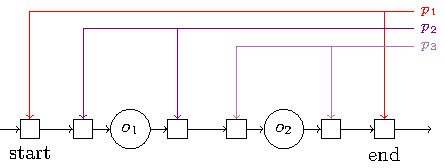
\includegraphics[scale=1.3]{tikz/probe_1.pdf}
            \end{center}
            \label{fig:probes_o}
            \caption{Probes inserted in the outcome diagram of the previous component diagram. \cref{fig:probes}}
        \end{figure}
       
       As for operators, probes are automatically attached to the components inside them and to the start event and end events of the operators. 

       \begin{figure}[H]
           \begin{center}
                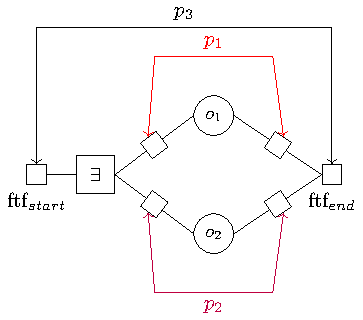
\includegraphics[scale = 1.3]{tikz/probe_2.pdf}
            \end{center}
            \label{fig:probes_op}
            \caption{Probes inserted into an operator.}
       \end{figure}
    
    The \textbf{observed $\Delta$Q} for the first-to-finish operator is the $\Delta$Q from the instances (\textbf{start}, \textbf{end}). The \textbf{calculated $\Delta$Q} is the $\Delta$Q which is the result of the first-to-finish operator being applied on $o_1, o_2$
        

